\section{Introduction}
An area where the chain rule is used extensively is deep learning, where the function value \( y \) is computed as a many-level function composition:
\[ 
y = (f_K \circ f_{K-1} \circ \cdots \circ f_1)(x) = f_K(f_{K-1}(\cdots (f_1(x)) \cdots )),
\]
where \( x \) are the inputs (e.g., images), \( y \) are the observations (e.g., class labels), and every function \( f_i \), \( i = 1, \ldots, K \), possesses its own parameters.

\begin{figure}[h]
	\centering
	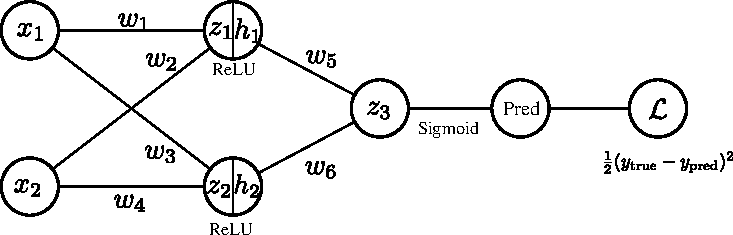
\includegraphics[scale=1.0]{./images/backprop.pdf}
\end{figure}

We have:

\begin{itemize}
	\item Inputs: $x_1, x_2$.
	\item Hidden layer: 2 neurons, each with no bias (for simplicity).  
	\item Weights $w_1, w_2, w_3, w_4, w_5, w_6$
	\item Output layer: 1 neuron, also with no bias.  
\end{itemize}

Where:
\begin{itemize}
	\item $z_1 = w_1 \, x_1 + w_2 \, x_2,\quad h_1 = \text{ReLU}(z_1)$
	\item $z_2 = w_3 \, x_1 + w_4 \, x_2,\quad h_2 = \text{ReLU}(z_2)$
	\item $z_3 = w_5 \, h_1 + w_6 \, h_2,\quad y_{\text{pred}} = \sigma(z_3)$
\end{itemize}

\begin{align*}
	\sigma(z) = \frac{1}{1 + e^{-z}}.
\end{align*}

We will train on one example $\{x=[x_1, x_2], y_\text{true}\}$.

% ---

% ## 2. Chosen Numerical Example

% - **Single training sample**:  
%   \(\displaystyle x_1 = 1.0,\quad x_2 = 0.0,\quad y_{\text{true}} = 1.0.\)
  
% - **Initial weights** (just for demonstration):  
%   \[
%     w_1 = 0.5, \quad w_2 = -0.5, \quad
%     w_3 = 0.3, \quad w_4 =  0.1, \quad
%     w_5 = 0.2, \quad w_6 = -0.1.
%   \]

Loss function: Mean Squared Error (MSE) for one sample:
  \[
    L = \frac{1}{2}\,\bigl(y_{\text{pred}} - y_{\text{true}}\bigr)^2.
  \]

We want to find the partial derivatives:

\begin{align*}
  \frac{\partial L}{\partial w_1},\;
  \frac{\partial L}{\partial w_2},\;
  \frac{\partial L}{\partial w_3},\;
  \frac{\partial L}{\partial w_4},\;
  \frac{\partial L}{\partial w_5},\;
  \frac{\partial L}{\partial w_6}.
\end{align*}


Useful Derivatives:
\begin{itemize}
	\item Derivative of the MSE loss (single sample):
	   \[
		 \frac{\partial L}{\partial y_{\text{pred}}}
		 = \bigl(y_{\text{pred}} - y_{\text{true}}\bigr).
	   \]
	\item Sigmoid derivative:
	   \[
		 \frac{d}{dz}\,\sigma(z) = \sigma(z)\,\bigl(1 - \sigma(z)\bigr).
	   \]
	   So,
	   \[
		 \frac{\partial y_{\text{pred}}}{\partial z_3} 
		 = y_{\text{pred}}\,(1 - y_{\text{pred}}).
	   \]
	\item Chain rule:  
	   \[
		 \frac{\partial L}{\partial z_3}
		 = \frac{\partial L}{\partial y_{\text{pred}}}
		   \;\times\; \frac{\partial y_{\text{pred}}}{\partial z_3}.
	   \]
\end{itemize}

The output node has:

\[
  z_3 = w_5\,h_1 + w_6\,h_2,
  \quad
  y_{\text{pred}} = \sigma(z_3).
\]

First, find \(\frac{\partial L}{\partial z_3}\):  
  \[
    \frac{\partial L}{\partial z_3}
    = (y_{\text{pred}} - y_{\text{true}}) \;\times\; 
      \bigl[y_{\text{pred}}\,(1 - y_{\text{pred}})\bigr].
  \]

Then,
  \[
    \frac{\partial L}{\partial w_5}
    = \frac{\partial L}{\partial z_3} \times \frac{\partial z_3}{\partial w_5}
    = \frac{\partial L}{\partial z_3} \times h_1.
  \]
Since \(z_3 = w_5\,h_1 + w_6\,h_2\), so \(\partial z_3/\partial w_5 = h_1\).

Each hidden neuron influences the output via \(h_1\) or \(h_2\). Let’s do them one neuron at a time.

#### 4.3.1. Hidden Neuron 1 (\(w_1, w_2\))

\[
  z_1 = w_1\,x_1 + w_2\,x_2,
  \quad
  h_1 = \sigma(z_1).
\]

To get \(\tfrac{\partial L}{\partial w_1}\), we chain through:

\[
  \frac{\partial L}{\partial w_1}
  = \frac{\partial L}{\partial z_3} 
    \,\times\, \frac{\partial z_3}{\partial h_1}
    \,\times\, \frac{\partial h_1}{\partial z_1}
    \,\times\, \frac{\partial z_1}{\partial w_1}.
\]

- We already have \(\frac{\partial L}{\partial z_3} = -0.12058.\)
- \(\frac{\partial z_3}{\partial h_1} = w_5\) (since \(z_3 = w_5\,h_1 + w_6\,h_2\)).
- \(\frac{\partial h_1}{\partial z_1} = \sigma(z_1)\bigl(1 - \sigma(z_1)\bigr) = h_1\,(1 - h_1)\).
- \(\frac{\partial z_1}{\partial w_1} = x_1\).

Numerically:

1. \(\frac{\partial z_3}{\partial h_1} = w_5 = 0.2.\)
2. \(h_1(1 - h_1) = 0.62246 \times (1 - 0.62246) = 0.62246 \times 0.37754 \approx 0.2350.\)
3. \(x_1 = 1.0.\)

So,

\[
  \frac{\partial L}{\partial w_1}
  = (-0.12058)\times(0.2)\times(0.2350)\times(1.0).
\]
Compute step by step:

- \((-0.12058)\times 0.2 = -0.024116.\)
- \((-0.024116)\times 0.2350 \approx -0.005667.\)

Thus,

\[
  \frac{\partial L}{\partial w_1} \approx -0.005667.
\]

For \(w_2\), the only difference is \(\frac{\partial z_1}{\partial w_2} = x_2\). Since \(x_2 = 0.0\) in our example, it follows immediately:

\[
  \frac{\partial L}{\partial w_2} = 0.
\]

#### 4.3.2. Hidden Neuron 2 (\(w_3, w_4\))

\[
  z_2 = w_3\,x_1 + w_4\,x_2,\quad h_2 = \sigma(z_2).
\]
By the same chain rule:

\[
  \frac{\partial L}{\partial w_3}
  = \frac{\partial L}{\partial z_3}
    \,\times\, \frac{\partial z_3}{\partial h_2}
    \,\times\, \frac{\partial h_2}{\partial z_2}
    \,\times\, \frac{\partial z_2}{\partial w_3}.
\]

- We have \(\tfrac{\partial L}{\partial z_3} = -0.12058.\)
- \(\tfrac{\partial z_3}{\partial h_2} = w_6 = -0.1.\)
- \(\tfrac{\partial h_2}{\partial z_2} = h_2 (1 - h_2) = 0.57444\times 0.42556 \approx 0.24450.\)
- \(\tfrac{\partial z_2}{\partial w_3} = x_1 = 1.0.\)

So,

\[
  \frac{\partial L}{\partial w_3}
  = (-0.12058)\times(-0.1)\times(0.24450)\times(1.0).
\]
Compute step by step:

1. \((-0.12058)\times(-0.1) = 0.012058.\)
2. \(0.012058 \times 0.24450 \approx 0.002950.\)

Hence,

\[
  \frac{\partial L}{\partial w_3} \approx 0.002950.
\]

For \(w_4\), again \(\partial z_2/\partial w_4 = x_2 = 0\), so:

\[
  \frac{\partial L}{\partial w_4} = 0.
\]

---

## 5. Weight Update

Let’s do **one step** of Gradient Descent with learning rate \(\eta = 0.1\). The update rule is:

\[
  w_i \;\leftarrow\; w_i \;-\; \eta\,\frac{\partial L}{\partial w_i}.
\]

### 5.1. Final Gradients Recap

- \(\displaystyle \frac{\partial L}{\partial w_1} \approx -0.005667\)  
- \(\displaystyle \frac{\partial L}{\partial w_2} = 0\)  
- \(\displaystyle \frac{\partial L}{\partial w_3} \approx 0.002950\)  
- \(\displaystyle \frac{\partial L}{\partial w_4} = 0\)  
- \(\displaystyle \frac{\partial L}{\partial w_5} \approx -0.07509\)  
- \(\displaystyle \frac{\partial L}{\partial w_6} \approx -0.06930\)

### 5.2. Updated Weights

1. \(\displaystyle w_1\):
   \[
     w_1 \leftarrow 0.5 - 0.1\times(-0.005667)
           = 0.5 + 0.0005667
           \approx 0.50057.
   \]

2. \(\displaystyle w_2\):
   \[
     w_2 \leftarrow -0.5 - 0.1\times 0 \;=\; -0.5.
   \]

3. \(\displaystyle w_3\):
   \[
     w_3 \leftarrow 0.3 - 0.1\times(0.002950)
           = 0.3 - 0.000295
           \approx 0.299705.
   \]

4. \(\displaystyle w_4\):
   \[
     w_4 \leftarrow 0.1 - 0.1\times 0 = 0.1.
   \]

5. \(\displaystyle w_5\):
   \[
     w_5 \leftarrow 0.2 - 0.1\times(-0.07509)
           = 0.2 + 0.007509
           \approx 0.20751.
   \]

6. \(\displaystyle w_6\):
   \[
     w_6 \leftarrow -0.1 - 0.1\times(-0.06930)
           = -0.1 + 0.00693
           \approx -0.09307.
   \]

---

## Recap

1. **Forward pass**:  
   - Calculated hidden neurons \(z_1, z_2\), then \(h_1, h_2\).  
   - Calculated output \(z_3\), then \(y_{\text{pred}}\).  
   - Computed the MSE loss \(L\).

2. **Backward pass**:  
   - Used the chain rule to find \(\tfrac{\partial L}{\partial w_i}\) for each weight.  
   - Observed how zero input (\(x_2=0\)) caused some gradients to be zero for this training example.

3. **Gradient Descent update**:  
   - Applied \(w_i \leftarrow w_i - \eta\,(\partial L/\partial w_i)\) with \(\eta=0.1\).

While we only did one training example and one update step, the principle is the same for multiple samples (you would sum or average the gradients across the batch). Larger networks just repeat the same chain-rule logic on more layers and neurons.

**That’s it!** This is the backpropagation process laid out in a small, fully traceable network with two hidden neurons. By doing the arithmetic yourself, you can see exactly how each weight nudges the output and how the gradients flow backward to update those weights.

